\documentclass[12pt]{article}
\usepackage[a4paper, total={6in, 10in}]{geometry}

\usepackage{graphicx}
\usepackage{abstract}
\usepackage{hyperref}
\usepackage{listings}
\usepackage{indentfirst}
\usepackage{amssymb}
\usepackage{titling}
\usepackage{mwe}
\usepackage{fancyhdr}
\usepackage{setspace}

\graphicspath{ {./images/} }
\renewcommand{\abstractname}{\small{\begin{center}Timestamps\end{center}\vspace{-4ex}}}

\setlength{\parskip}{3mm}   % Add space between paragraphs.
\setlength{\parindent}{0.5in}
\setlength{\droptitle}{-35pt}
\onehalfspacing

\fancypagestyle{plain}{
    \vspace{3ex}
    \fancyhead[L]{November 14th, 2020}
    \renewcommand{\headrulewidth}{0.5pt}
}

\pretitle{\begin{center} \LARGE \textbf}
\posttitle{\end{center} \vspace{-3ex}}
\preauthor{\begin{center} \large}
\postauthor{\end{center} \vspace{-3ex}}
\predate{\begin{center} \small \emph}
\postdate{\end{center} \vspace{-3ex}}

\title{Chapter 8 \& 9 Summary}
\author{Chris Nutter\thanks{Dedicated to @QuesoGrande a.k.a. Jared D.}}
\date{CPSC 315}

% --> Here we go, satellite radio, y'all get hit with a...

\begin{document}
\maketitle

%\begin{center} \vspace{-4ex}|\vspace{-3ex} \end{center}

\noindent\abstractname
\begin{center}
    \normalsize\textbf{10/08/2020 - 01:58:55 PM}\\
    Figures of each model are at the end of the document.
\end{center}
\normalsize

\tableofcontents    
\vspace{4ex}

% --> First Chapter

\section{Chapter 8 Summary}
    \indent Having software requirements is a main staple for a good engineering ethic. If you do not have a proper set of requirements for engineers to implement, there is no purpose or drive to products and they are created on a whim (which isn't necessarily bad but it isn't proper). Requirements are designed to be showcased before starting and demonstrate a foundation for a project.  

\end{document} 

% Possibly Important LaTeX Functions %
% ================================== %

%   \begin{figure}[hbtp]
%       \centering
%       \fbox{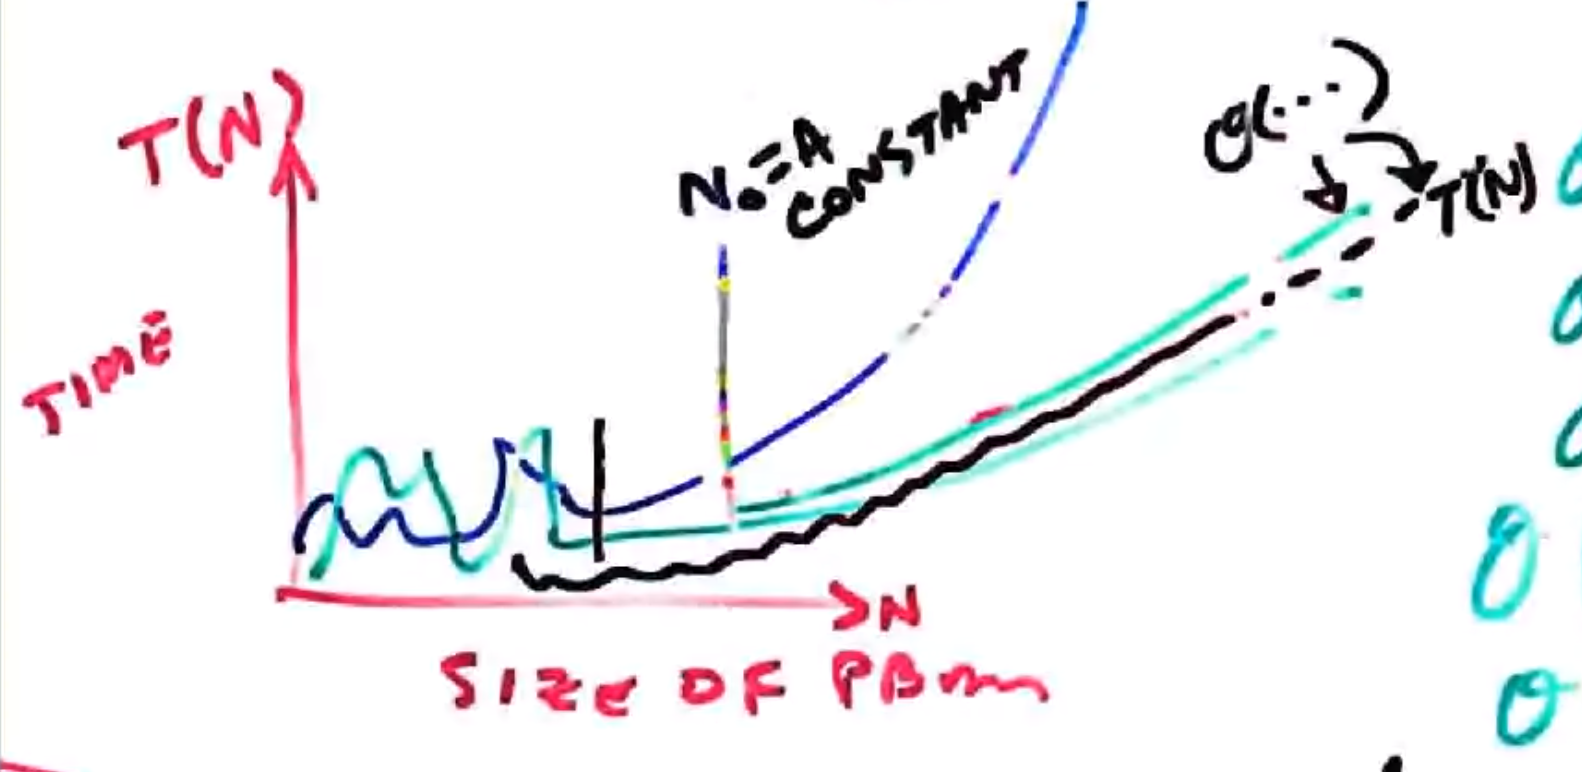
\includegraphics[width=13.8cm]{big_o.png}}
%       \caption{Big(O) Notation}
%   \end{figure}

%   \begin{lstlisting}[language=Python] 
%        print('hello world') 
%   \end{lstlisting}  

